%%%%%%%%%%%%%%%%%%%%%%%%%%%%%%%%%%%%%%%%%
% Journal Article
% LaTeX Template
% Version 1.3 (9/9/13)
%
% This template has been downloaded from:
% http://www.LaTeXTemplates.com
%
% Original author:
% Frits Wenneker (http://www.howtotex.com)
%
% License:
% CC BY-NC-SA 3.0 (http://creativecommons.org/licenses/by-nc-sa/3.0/)
%
%%%%%%%%%%%%%%%%%%%%%%%%%%%%%%%%%%%%%%%%%

%----------------------------------------------------------------------------------------
%	PACKAGES AND OTHER DOCUMENT CONFIGURATIONS
%----------------------------------------------------------------------------------------

\documentclass{article}

%\documentclass{aastex}  % version 5.0 or prior
%\usepackage{natbib}



\usepackage{graphicx}
\usepackage{lipsum} % Package to generate dummy text throughout this template
%\usepackage[sc]{mathpazo} % Use the Palatino font
\usepackage[T1]{fontenc} % Use 8-bit encoding that has 256 glyphs
\linespread{1.05} % Line spacing - Palatino needs more space between lines
\usepackage{microtype} % Slightly tweak font spacing for aesthetics

\usepackage[margin=1in,columnsep=20pt]{geometry} % Document margins
\usepackage{multicol} % Used for the two-column layout of the document
\usepackage[hang, small,labelfont=bf,up,textfont=it,up]{caption} % Custom captions under/above floats in tables or figures
\usepackage{booktabs} % Horizontal rules in tables
\usepackage{float} % Required for tables and figures in the multi-column environment - they need to be placed in specific locations with the [H] (e.g. \begin{table}[H])
\usepackage{hyperref} % For hyperlinks in the PDF
\usepackage{subcaption}

\usepackage{lettrine} % The lettrine is the first enlarged letter at the beginning of the text
\usepackage{paralist} % Used for the compactitem environment which makes bullet points with less space between them
\usepackage{amsmath}
\usepackage{abstract} % Allows abstract customization
\renewcommand{\abstractnamefont}{\normalfont\bfseries} % Set the "Abstract" text to bold
\renewcommand{\abstracttextfont}{\normalfont\small\itshape} % Set the abstract itself to small italic text

\usepackage{titlesec} % Allows customization of titles
%\renewcommand\thesection{\Roman{section}} % Roman numerals for the sections
%\renewcommand\thesubsection{\Roman{subsection}} % Roman numerals for subsections
%\renewcommand\thesubsubsection{\Alph{subsubsection}} % Roman numerals for subsections
\titleformat{\section}[block]{\Large\scshape}{\thesection}{1em}{} % Change the look of the section titles
\titleformat{\subsection}[block]{\large}{\thesubsection}{1em}{} % Change the look of the section titles
\titleformat{\subsubsection}[block]{}{\thesubsubsection}{1em}{} % Change the look of the section titles

\usepackage{fancyhdr} % Headers and footers
\pagestyle{fancy} % All pages have headers and footers
\fancyhead{} % Blank out the default header
\fancyfoot{} % Blank out the default footer
\fancyhead[C]{Montana State University \quad $\bullet$ \quad CSCI 466 Artificial Intelligence \quad $\bullet$ \quad Group 21} % Custom header text
\fancyfoot[RO,LE]{\thepage} % Custom footer text

\newcommand{\ve}[1]{\boldsymbol{\mathbf{#1}}}

%----------------------------------------------------------------------------------------
%	TITLE SECTION
%----------------------------------------------------------------------------------------

\title{\vspace{-15mm}\fontsize{24pt}{10pt}\selectfont\textbf{CSCI 446 Artificial Intelligence \\ Project 1 Design Report} \\[-2mm]} % Article title
\date{\today}
\author{
\large
\textsc{Roy Smart} \and \textsc{Nevin Leh} \and \textsc{Brian Marsh}\\[2mm] % Your name
}


%----------------------------------------------------------------------------------------

\begin{document}

\maketitle % Insert title

\thispagestyle{fancy} % All pages have headers and footers

%\begin{abstract}
%We present a novel way of performing MOSES data inversions using a
%\end{abstract}

%----------------------------------------------------------------------------------------
%	ARTICLE CONTENTS
%----------------------------------------------------------------------------------------

\begin{multicols}{2} % Two-column layout throughout the main article text
\normalsize
\section{Introduction}
The \textit{Graph Coloring Problem} (GCP) is the problem of attempting to color a set of interconnected regions such that no region has the same color as its neighbors using three or four colors. For example consider the problem of coloring a map of the USA (Figure \ref{usa}), using only four colors and ensuring that no neighboring states share the same color. This is the motivation of the graph coloring problem. 
\begin{figure}[H]
	\centering
	\includegraphics[width=\linewidth]{images/usa}
	\caption{Map of the United States of America satisfying the graph coloring problem.}
	\label{usa}
\end{figure}
It can be shown that the map coloring problem reduces to the graph coloring problem if we represent the states as the vertices of the graph, and the borders between states as the edges of the graph\cite{ai}. This configuration produces a \textit{planar} graph, a graph with no edge intersections. 
\begin{figure}[H]
	\centering
	
\includegraphics[width=0.4\linewidth]{images/simple_graph}
	\caption{Simple example of a maximally planar graph.}
	\label{simple}
\end{figure}
For this project, we will concentrate on solving the graph coloring problem for \textit{maximally planar} graphs (Figure \ref{simple}), planar graphs for which adding any addition edge would make the graph non-planar.

We are tasked with solving the GCP five different ways: Minimum Conflicts, Simple Backtracking, Backtracking with Forward Checking, Backtracking with Constraint Propagation (MAC), and Local Search using a Genetic Algorithm. To test these algorithms, we will first need to build a problem generating program that can produce a random set of maximally planar graphs. Using the problem generator, we will calculate a set of graphs between the sizes \{10, 20, 30,...,100\} and then use the five graph coloring algorithms to solve the GCP. We will measure GCP algorithm performance by how many vertex read/write operations it requires to find a solution.  \par The solution to this project will be implemented in Python 3.4 using the graphics library to visualize the graphs.
\section{Problem Generation}
\subsection{Computing a Maximally Planar Graph}
For this project, we will need to create maximally planar graphs (MPGs) from a set of randomly scattered points. For an arbitrary set of points, there is no unique MPG that can be constructed. To solve this issue, the problem statement has provided a prescription for calculating an MPG. 
\begin{quote}
Select some point $X$ at random and connect $X$ by a straight line
to the nearest point $Y$ such that $X$ is not already connected to $Y$ and line crosses no other line. Repeat the
previous step until no more connections are possible.
\end{quote}
To implement this algorithm we will first create a complete graph (where each vertex is connected to every other vertex). Each vertex will have a list of associated edges, sorted by length. As instructed, we will then select a point at random and inspect the first unchecked edge $E$. If $E$ doesn't cross any of the accepted edges, it is added to the list of accepted edges and marked as checked. We then repeat this process until every edge has been checked. \par
An algorithm to determine if two edges (or line segments) cross has been outlined by LaMothe \cite{tricks} and described in detail here. Let's start by defining two line segments 
\begin{align}
	\begin{split}
		& A = \{ \ve{a},\; \ve{a'} \} \\
		& B = \{\ve{b}, \;\ve{b'}\}
	\end{split}
\end{align}
where $\ve{a}, \; \ve{a'}, \; \ve{b}, \text{ and } \ve{b'}$ are vectors from the origin to the ends of the line segments. Next, compute the direction vectors for each line segment
\begin{align}
	\begin{split}
		&\ve{\alpha} = \ve{a}' - \ve{a} \\
		&\ve{\beta} = \ve{b}' - \ve{b} 
	\end{split}
\end{align}
Now, the trick to solving this problem is to parameterize the line segment using the direction vector and a parameter $t_i$ in the domain $[0, \; 1]$.
\begin{align}
	\begin{split}
		& \ve{p} = \ve{a} + \ve{\alpha} t_a, \quad t_a \in [0, \; 1]\\
		& \ve{q} = \ve{b} + \ve{\beta} t_b, \quad t_b \in [0, \; 1]
	\end{split}
\end{align}
From here, the solution is obvious. To find the point of intersection, we set $\ve{p} = \ve{q}$ and solve for the values of $t_a$ and $t_b$. Then, if the solution is outside the domain of $t_i$, the line segments do not intersect. Thus,
\begin{align}
	\Rightarrow \; &\begin{cases}
		p_x = q_x \\
		p_y = q_y
	\end{cases} \\
	\Rightarrow \; & \begin{cases}
		a_x + \alpha_x t_a = b_x + \beta_x t_b \\
		a_y + \alpha_y t_a = b_y + \beta_y t_b.
	\end{cases} \label{system}	
\end{align}
Equation \ref{system} is a system of two equations and two unknowns, solving for $t_a$ and $t_b$ gives
\begin{align}
	\Rightarrow \; & \begin{split}
		&t_a = \frac{(-a_y + b_y)\beta_x + (a_x - b_x)\beta_y}{\alpha_y \beta_x - \alpha_x \beta_y} \\
		&t_b = \frac{(a_y - b_y)\alpha_x + (-a_x + b_x)\alpha_y}{-\alpha_y \beta_x + \alpha_x \beta_y}.
	\end{split}
\end{align}
Finally, we can determine whether $A$ and $B$ intersect if $0 < t_a < 1$ and $0 < t_b < 1$ evaluates to true. \par
Utilizing the algorithms described above we have implemented problem generation code in Python to compute MPGs of arbitrary size. The output of a random execution of the problem generator is shown in Figure \ref{graph_ex}
\begin{figure}[H]
	\centering
	\includegraphics[trim={0 4cm 0 0.5cm},clip,width=0.9\linewidth]{images/graph_example}
	\caption{Example of the MPG produced by our problem generator code with the number of vertices, $N=10$.}
	\label{graph_ex}
\end{figure}
\subsection{Computing Vertex Polygons}
We have also implemented a way to produce a map of regions that is analogous to the graphs created by the problem generator, shown in Figure \ref{poly_ex}.  
\begin{figure}[H]
	\centering
	\includegraphics[width=0.9\linewidth]{images/poly_example}
	\caption{The example of Figure \ref{graph_ex}, overlaid with the regions corresponding to each vertex. Each vertex has been randomly colored in this example.}
	\label{poly_ex}
\end{figure}
Since the graph coloring problem does not uniquely define the map coloring problem, we had to invent a metric that produces appropriate graphs. To define our metric, consider that if a polygon $G_i$ corresponding to each point $P_i$ were constructed out of the midpoints $M_{i,m}$ of the associated edges $E_{i,m}$ of $P_i$, then an adjacent polygon $G_j$ would only touch at the corners, that is, our map would be full of gaps. Therefore, to fix the problem we also define the centroid $C_{i,n}$ of each triangle $T_{i,n}$ formed by the two adjacent edges $E_{i,m}$ and $E_{i,m+1}$. We then define the final polygon for $P_i$ using the points $M_{i,m}$ and $C_{i,n}$. This procedure is unnecessary in terms of the assignment, but is helpful for debugging and for aesthetic pleasure.

\section{Experiment Design}
\subsection{Invariant Metrics}
Our goal with this project is to solve the graph coloring problem using five different algorithms while comparing the relative performance of each algorithm. Since CPU time and wall-clock time are not reliable measurements of computation, we will have to define a metric that allows us to compare different algorithms.\par  We propose to solve this problem using the concept of counting vertex read/write operations. The procedure will be to tally how many times each algorithm peeks into a vertex to determine its color and also how many times the algorithm must poke a vertex to update its color. This metric has the advantage of being algorithm independent, since all of our algorithms need the ability to set vertex colors and check the colors of adjacent vertices.\par
To acquire good performance statistics we will run ten experiments on each of the ten possible values for $N$ (10, 20, 30, 40, 50, 60, 70, 80, 90, 100) using each of the five GCP algorithms for a total of 500 experiments. We will then plot the average number of total vertex reads/writes vs $N$ for each algorithm. These graphs will allow us determine relative algorithm performance and also the time complexity, $\mathcal{O}$, of each GCP algorithm.
\subsection{Algorithm-Specific Metrics}
\section{Software Design}
We will use Python 3.4 for this project as it has simple graphics support for program testing, object-oriented paradigms, and convenient ways of parsing and storing data structures. The program entry point is the \texttt{Main} function. This function will be responsible for generating the datasets, managing the experiments, collecting results, and displaying the output.
\begin{figure}[H]
	\centering
	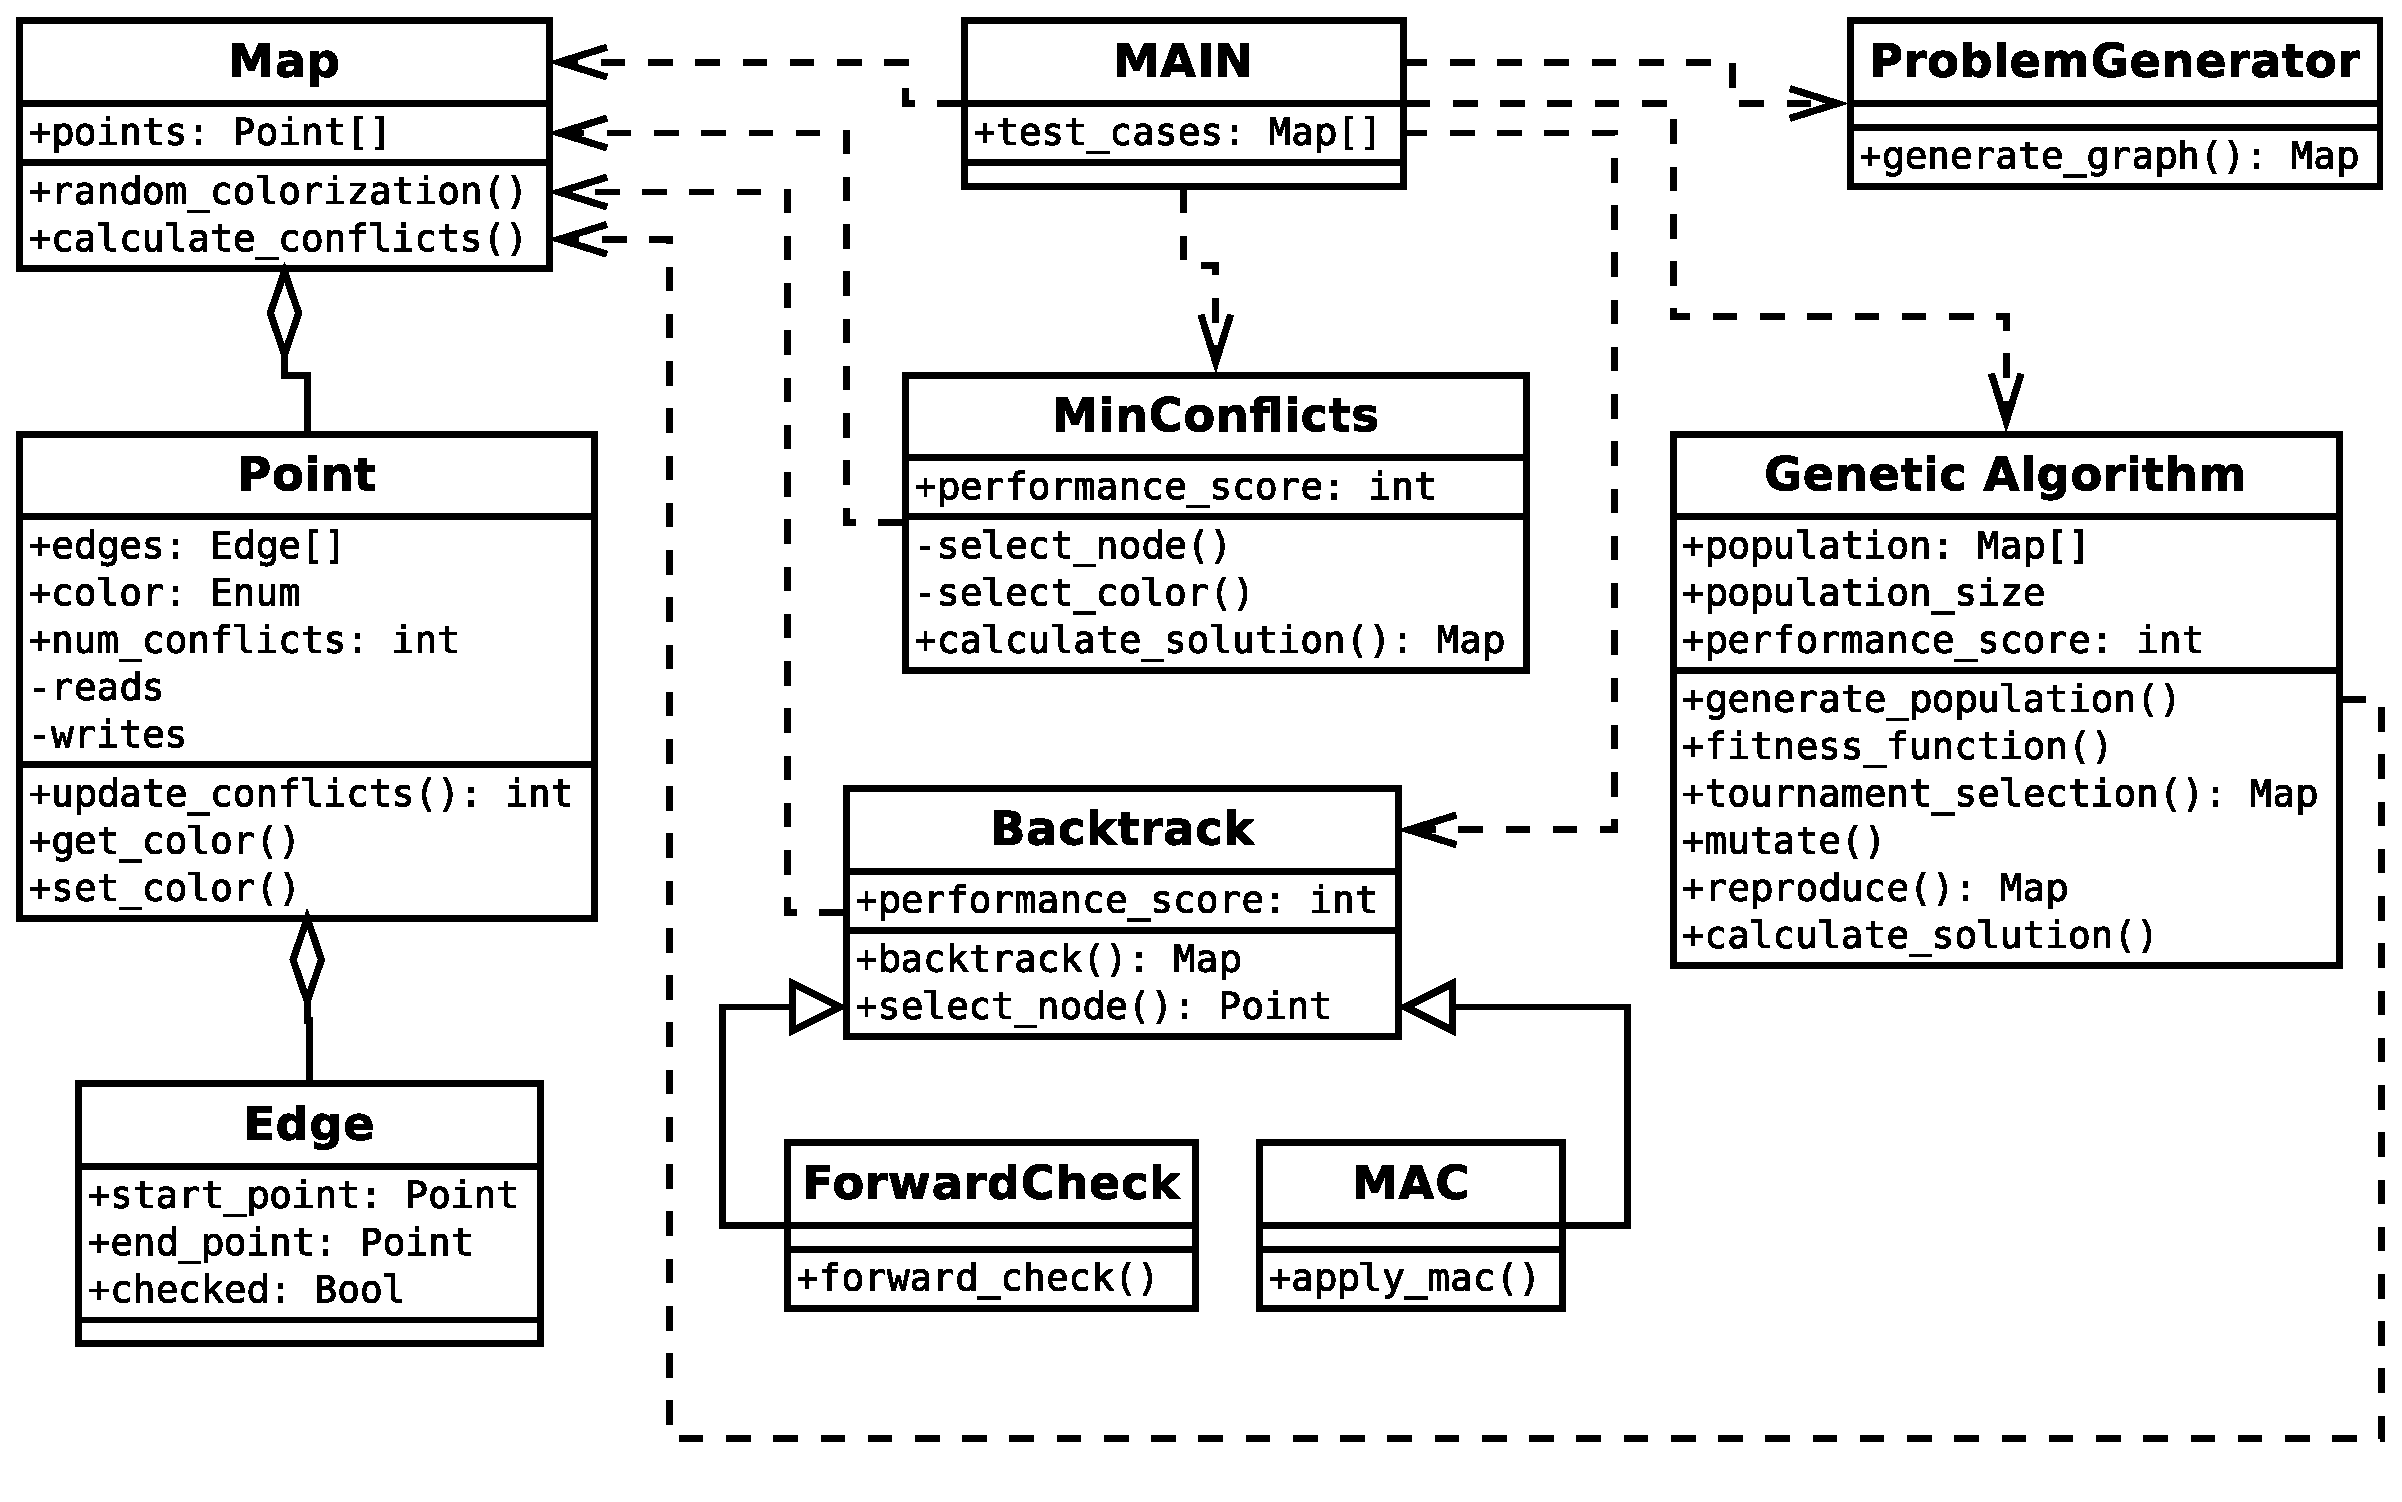
\includegraphics[width=\linewidth]{images/AI_UML_Project_1}
	\caption{A UML diagram describing the objects that each algorithm will use to solve the GCP and their relationships.}
	\label{uml}
\end{figure}
\section{GCP Algorithms}
\subsection{Minimum Conflicts}
Minimum conflicts is a local search algorithm that can be used to solve the graph coloring problem. The approach is to randomly color the graph and assign each node a conflict score determined by how many of its neighbors have a color in common with that node. The algorithm then randomly chooses a conflicting node and changes it to a color that results in the least conflicts. The algorithm continues to choose conflicting nodes and changing them until there are no more conflicts or an until a predefined limit on how long the program runs is reached \cite{ai}. \par
There are several design decisions that have been made to facilitate the use of this algorithm. One decision is to include a conflict score variable with each point. In addition, some functions will have to be implemented such as a node selector that ignores nodes with zero conflicts and a function that selects a color that causes the least amount of conflicts.
\subsection{Simple Backtracking}
Backtracking is a variant of the depth-first search. For the graph coloring problem the approach is to choose a node and assign it a valid color. The algorithm continues to do this until a solution is found or a node is reached that cannot be assigned a valid color. If the node cannot be assigned a valid color the algorithm back tracks to the previous node and tries a different color.  \par
This algorithm will have several design features that are required to make the algorithm work. The foremost feature is that the algorithm will be recursive as it is a convenient way of keeping track of old states. Each instance of the recursive function will have a list of previously used colors so it can know when to backtrack. The experimental design will consist of a counter that is incremented each time a node is colored. 
\subsection{Backtracking with Forward Checking}
\subsection{Backtracking with Constraint Propagation}
\subsection{Local Search using a Genetic Algorithm}


\end{multicols}

	%\bibliographystyle{apj}
	\bibliographystyle{unsrt}
	\bibliography{sources}
\end{document}